% Manuscript source. Build with pdflatex/bibtex (or latexmk). Quantitative
% statements are tied to the archived analysis outputs, with scope and limits
% stated alongside each claim.
\documentclass[aps,pre,twocolumn,superscriptaddress,floatfix,nofootinbib]{revtex4-2}

\usepackage{amsmath,amssymb,bm}
\usepackage{graphicx}
\usepackage[colorlinks=true,allcolors=blue]{hyperref}

\newcommand{\eps}{\varepsilon}
\newcommand{\avg}[1]{\left\langle #1 \right\rangle}
\newcommand{\Teff}{T_{\mathrm{eff}}}
\newcommand{\Var}{\mathrm{Var}}

\begin{document}

\title{Signed order flow as a transport current:\\
response, noise and counting statistics of a driven market}

\author{Nelson Bol\'{\i}var}
\affiliation{Escuela de F\'isica, Facultad de Ciencias, Universidad Central de Venezuela, Caracas 1041-A, Venezuela}
\affiliation{Astrum Drive Technologies, 13024 Dallas Pkwy Unit 120 B, Frisco, TX 75034, USA}
\author{Gabriel Abell\'an}
\affiliation{Escuela de F\'isica, Facultad de Ciencias, Universidad Central de Venezuela, Caracas 1041-A, Venezuela}
\affiliation{Astrum Drive Technologies, 13024 Dallas Pkwy Unit 120 B, Frisco, TX 75034, USA}
\author{David Verrilli}
\affiliation{Escuela de F\'isica, Facultad de Ciencias, Universidad Central de Venezuela, Caracas 1041-A, Venezuela}

\date{\today}

\begin{abstract}
We measure the full counting statistics of signed order flow, treating it as
the transferred charge of an open conductor, and find that it is strongly
bunched: the Fano factor is of order $10^{3}$ and grows as
$T^{0.19\text{--}0.28}$ with the counting window, while the counting variance
grows superdiffusively with an exponent of $1.10$--$1.43$, robust across
estimators built to be blind to a drifting mean.
Neither number is reachable by any free-fermion counting problem, for which
Pauli statistics bound the Fano factor below unity and the variance grows
diffusively; the bunching therefore localises the missing physics in the
interaction between flow and available liquidity rather than in the transport
itself. Establishing this requires separating it from what is \emph{not}
informative, which is our second contribution. Carrying out the full transport
programme on the same data --- current, impact response, noise, counting,
affinity, two-time structure after a shock, and response to periodic driving ---
partitions the problem into three sectors with three different statuses. The
second-order sector closes but is empty: the counting variance reproduces the
independently measured autocorrelation to within $4\%$ across $64$
window--series combinations, and the linear fluctuation symmetry with slope
$2\avg{Q}/\Var(Q)$ that this sector exhibits is an algebraic identity for any
Gaussian variable, not evidence of a nontrivial fluctuation theorem. The
response sector is explained by the price integrating the unpredictable part of
the flow. Two further constraints on any model follow: the mean flow ages after
a large shock while the correlation does not, and bias, affinity and impact all
modulate with the daily cycle in every asset tested. The first of these carries
a methodological result we report in its own right, because the correlation
initially appeared to age with a rank correlation of $+1.00$ across age bins:
normalising a post-event signal by a pre-event quantity manufactures ageing by
construction, and randomly placed events reproduce the same monotone growth
exactly. We use four cryptocurrency pairs over four years, and document the
inference pitfalls that arose along the way, several of which produced results
we would otherwise have believed.
\end{abstract}

\maketitle

\section{Introduction}

A market has two sides. Buyers and sellers meet through an order book, and the
net signed flow of executed orders is a current in the ordinary sense: it counts
something that moves from one side to the other, it fluctuates, and it responds
to the conditions that drive it. This is not a metaphor we intend to defend on
aesthetic grounds. It is a claim that a specific and well-developed measurement
programme --- the one built for transport in open, driven, mesoscopic systems ---
can be carried out on market data, and that carrying it out completely tells us
something that measuring any one piece of it does not.

That programme has a standard shape. One measures the current, then the linear
response of the system to the drive, then the noise, and then --- the part that
is genuinely informative and usually the hardest --- the full counting
statistics of the charge transferred in a finite window, including the higher
cumulants and the symmetry of the distribution under reversal of the counted
charge. Each layer constrains the next. Our purpose here is to do all of it on
the same data set, with the same conventions, so that the layers can be
compared rather than quoted in isolation.

\paragraph*{What is already known, and what we are not claiming.}
We want to be precise about our position in a crowded neighbourhood, because
several nearby framings are already occupied and it would be easy to appear to
be claiming them.

Statistical-physics readings of markets are not new. Effective temperatures
have been defined from the ratio of positive to negative returns
\cite{ramezani2025}, from the kinetic and potential energies of the limit order
book \cite{li2024entropy}, and from asymmetries in position holding times
\cite{gao2026}; fluctuation relations have been examined for volatility
cascades. Closest to our observables, Yura \textit{et al.}\ \cite{yura2014}
studied the order book as a colloidal fluid surrounding an effective Brownian
particle and reported that a fluctuation--dissipation relation \emph{holds},
with an inner layer of short memory and an outer layer of long memory. We
measure a fluctuation--dissipation ratio that is manifestly \emph{not} constant.
The two results are not in conflict --- they concern different observables (the
midprice particle versus the signed flow as a current) --- but the difference is
sharp enough that we flag it here rather than leave it for the reader to
discover.

Likewise, the persistence of order flow and its coexistence with nearly
martingale prices is long understood, and its microscopic origin in order
splitting is by now quantitatively established
\cite{lillo2005,sato2023prl,sato2023prr}. The resolution --- prices respond to
the surprise in the flow rather than to the flow itself --- is not ours. It is
stated as a theorem in the history-dependent impact model of Taranto
\textit{et al.}\ \cite{taranto2016}, where $r_t = G(1)\,(\eps_t-\hat\eps_t) +
\eta_t$ with $\hat\eps_t$ the linear predictor of the sign, so that the price
is an exact martingale by construction; the decaying propagator and the
innovation representation are the same object written twice, the propagator
kernel being the predictor coefficients with the sign reversed. We use this
below only as a check that our conventions are right.

Two further attributions are owed, and both cut close enough that we make them
before stating our own claim. First, the moments of the transferred flow are
\emph{not} unmeasured. Maitrier and Bouchaud \cite{maitrier2026} define the
generalised imbalance $I_T^{\,a} = \sum_t \eps_t\, q_t^{\,a}$ --- our $Q_T$ at
$a=1$ --- and give both its variance and its higher even moments as powers of
$T$, validated empirically to sixth order, attributing the anomalous scaling to
order splitting. Our Fano growth is an algebraic rewriting of that result, and
the underlying variance scaling is older still, implicit in the Hurst exponent
of Lillo and Farmer \cite{lillo2004}. Second, the log-ratio estimator of a
fluctuation symmetry has already been applied to markets: Ramezani
\textit{et al.}\ \cite{ramezani2025} write $P(+Q,\tau)/P(-Q,\tau) =
\exp(Q\,\Delta\beta)$ for returns, and Gao \textit{et al.}\ \cite{gao2026}
apply the same construction to position holding times. The technique is not
ours; the observable is.

We should also distinguish a nearby field-theoretic treatment. Shi
\textit{et al.}\ \cite{shi2021} build a non-equilibrium field theory of the
Bitcoin order book in which the net market-order discrepancy enters a
continuity equation as a boundary current driving the book's density field.
That is order flow as a current, in this asset class, in non-equilibrium
language. The object differs from ours: they model the density field of the
book and treat flow as its boundary source, whereas we treat the signed-flow
time series itself as the transport current and measure its memory kernel,
response and counting statistics.

What we claim is accordingly narrower than a new observable, and we think
stronger for being narrow. It is the \emph{joint and named} characterisation.
The pieces above were obtained along independent routes and in unrelated
vocabularies --- a propagator fitted by deconvolution, a Hurst exponent, a
branching ratio, a variance-to-mean ratio, a log-ratio slope --- and each was
reported without reference to the others. Read as transport they are the
Langreth components of one generating functional: the propagator is the
retarded response, the variance-to-mean ratio is a susceptibility, the
kernel-from-correlation inversion is a fluctuation--dissipation relation, and
the log-ratio slope is an affinity. Measuring them on one data set with one
set of conventions is what allows the three sectors of
Sec.~\ref{sec:discussion} --- closed, explained, open --- to be separated at
all, and separating them is the output of the paper. The specific quantities
we could not find measured for the signed flow are the odd cumulants, the
effective transfer quantum extracted from the Fano factor, and the
finite-frequency noise spectrum of the current.

\paragraph*{The central result.}
Since what follows is a systematic characterisation, it is worth saying at the
outset which part of it we regard as the finding and which part is scaffolding.

\emph{The finding is that the counting sector is strongly bunched, and bunched
beyond what free transport can produce.} The Fano factor is of order $10^{3}$
and grows with the counting window, and the counting variance grows
superdiffusively. A free-fermion counting problem cannot produce either: Pauli
statistics bound the Fano factor below unity, and single-channel transport with
finite memory gives diffusive growth. These are bounds on statistics, not on
parameters, so no choice of coupling, bias or temperature evades them. The
measured values therefore require both a heavy-tailed distribution of transfer
sizes, for the level, and genuine long memory, for the growth --- and they place
the missing ingredient in the interaction between order flow and available
liquidity, exactly where the microscopic order-splitting account puts it
\cite{lillo2005,sato2023prl}.

\emph{The scaffolding is everything that had to be measured to know that.} A
large Fano factor means little in isolation; it means something once one has
shown that the second-order sector closes trivially, that the response is
accounted for, that the correlation carries two decay regimes, and that the
observed affinity is what a Gaussian would give anyway. That is why we report
the whole programme rather than the one number, and why the partition into
three sectors --- closed and empty, explained, open --- is the organising output
of the paper.

\paragraph*{Why cryptocurrency, and what that costs.}
Three properties of these markets matter for this measurement. Public candle
data carry the taker-side volume directly, so the signed flow is recoverable
without proprietary feeds; trading runs continuously, so there are no overnight
gaps to interrupt two-time estimates or the daily-phase analysis; and four years
of hourly data give $3.5\times10^{4}$ observations per asset, which the counting
statistics need since the higher cumulants converge slowly under heavy tails.

The cost is generality. These are venues with their own microstructure, and the
order-splitting mechanism whose signature we find in the slow correlation regime
was established on equity markets \cite{lillo2005,sato2023prl,sato2023prr}. We
regard the mechanism as the universal part and the venue as incidental, but that
is an expectation and not something this data set can test. The statistical
statements below are about these four pairs.

\section{Data and base measurement}
\label{sec:data}

We use hourly and four-hourly candles for four cryptocurrency pairs (BTC, ETH,
BNB, SOL against USDT) over four years, $35\,063$ hourly and $8\,766$
four-hourly observations per asset. The signed flow follows directly from the
public candle fields as $\eps_t = 2\,V^{\rm taker\,buy}_t - V_t$, normalised by
volume; no proprietary data is required. Analysis code and all logs backing the
numbers below are available \cite{code_keldysh_finance}.

Three conventions matter enough to state explicitly.

\emph{Causality.} Every window is trailing. This is the property on which
everything else depends, and we test it directly: perturbing the future of the
series must leave past features numerically unchanged.

\emph{Alignment.} Flow features live on the candle index while returns are
differences of log prices, so the feature of candle $j$ corresponds to return
index $j-1$. Getting this offset wrong introduces look-ahead that no
window-based test detects, because the features do not move --- the labels do.

\emph{Sign of impact.} The impact of $\eps_t$ is already inside the closing
price of candle $t$, so referencing the response to $\log(\text{Close})$
measures the subsequent relaxation and returns a spurious negative impact. We
reference to the opening price.

\paragraph*{A limitation of public data, stated up front.}
Naviglio \textit{et al.}\ \cite{naviglio2025} show that impact estimated from
public market data is systematically distorted: models trained on public flow
produce price paths that rise linearly rather than concavely during execution
and revert too little afterwards, and they trace the problem to a
misattribution of the origin of order-flow autocorrelation. The warning applies
to our data source and we do not claim to evade it. What we would argue is that
it bites hardest on the quantity we are not estimating. We do not reconstruct
metaorders or measure their impact; we measure the aggregate response of the
price to the aggregate signed flow, together with the noise and counting
statistics of that flow. Those are properties of the public series itself
rather than inferences about hidden parent orders. The distinction matters for
Sec.~\ref{sec:counting}, whose observables involve no impact estimation at all,
and it should temper the reading of the response measurement in
Sec.~\ref{sec:data}, which is an aggregate lagged covariance and not a
metaorder impact curve.

\subsection{Memory of the flow, and why one exponent is not enough}
\label{sec:acf}

The flow autocorrelation $C_\eps(\tau)$ decays as a power law, and this is the
standard point of contact with the literature: order splitting predicts
long-memory signs \cite{lillo2005}, verified microscopically
\cite{sato2023prl,sato2023prr}. Fitting a single exponent over $60$ lags we
obtain $\gamma = -0.380 \pm 0.052$ (BTC) and $-0.474 \pm 0.052$ (ETH) at hourly
resolution, broadly consistent with the reported $\gamma\approx-0.5$.

That agreement, however, needs a caveat that turns out to organise much of this
paper. \emph{The single exponent is not well defined without declaring the lag
window}, because $C_\eps$ has two regimes. Fitting local slopes separately we
find, for the raw hourly series,
\begin{equation}
  a_f = 1.00\pm0.15,\; 0.87\pm0.08,\; 0.46\pm0.05,\; 1.72\pm0.23
\end{equation}
over $\tau\in[2,10]$ for BTC, ETH, BNB and SOL respectively, against
\begin{equation}
  a_s = 0.17\pm0.13,\; 0.22\pm0.09,\; 0.29\pm0.05,\; 0.16\pm0.32
\end{equation}
over $\tau\in[10,50]$. The fast regime is steeper than the slow one in all four
assets, though the values themselves vary considerably between assets and the
slow exponents carry large errors. A single-exponent fit over a wide window
returns something in between, which is why quoted values of $\gamma$ are
sensitive to the fitting range.

We checked whether the slow regime is an artefact of the daily periodicity
documented in Sec.~\ref{sec:floquet}: a periodic mean contributes a
non-decaying term to the autocorrelation and could masquerade as slow memory.
Removing the seasonal component barely moves the slopes (e.g.\ BTC:
$-1.003\to-0.941$ fast, $-0.168\to-0.212$ slow), so the slow regime is genuine
multi-day stochastic memory rather than the drive.

\subsection{Response and the fluctuation--dissipation ratio}
\label{sec:response}

The lagged impact $R(\tau)$ is nearly flat in $\tau$, in sharp contrast to
$C_\eps$, which falls by roughly an order of magnitude over the same range
[Fig.~\ref{fig:base}(a)]. Fitting a log-slope to $R$ gives values scattered
around zero and small compared with $\gamma$ --- e.g.\ $b_R = 0.064\pm0.006$
(BTC$\cdot$1h) and $0.094\pm0.008$ (ETH$\cdot$1h) --- though we note honestly
that some series depart from flatness at resolvable significance
($b_R = -0.149\pm0.017$ for BNB$\cdot$4h). ``Flat'' here means flat to within
about a tenth of the decay exponent of the correlation, not flat exactly.

Flat response is what the surprise mechanism predicts
\cite{gerig2008,jaisson2014,muhlekarbe2026}: if the price integrates the
unpredictable part of the flow, the predictable part moves nothing and the
lagged covariance saturates immediately. We recover it as a check on our
conventions, not as a result.

The consequence is that the fluctuation--dissipation ratio
\begin{equation}
  \Teff(\tau) \;\equiv\; -\,C'_\eps(\tau)\big/R(\tau)
\end{equation}
has essentially no shape freedom of its own: with $R$ flat, $\Teff$ simply
inherits the derivative of $C_\eps$ [Fig.~\ref{fig:base}(b)]. Reporting a single
scalar ``violation of the fluctuation--dissipation theorem'' is therefore
reporting one point of a curve. We give the curve.

Notably, a composite single-exponent form for $\Teff$ built from the
single-exponent $\gamma$ fails for all eight series, with discrepancies of
$2.0$ to $7.2$ standard deviations. This is not an estimator failure: it is what
Eq.~(1)--(2) demand, since a sum of two power laws is not a power law.

\begin{figure}[t]
  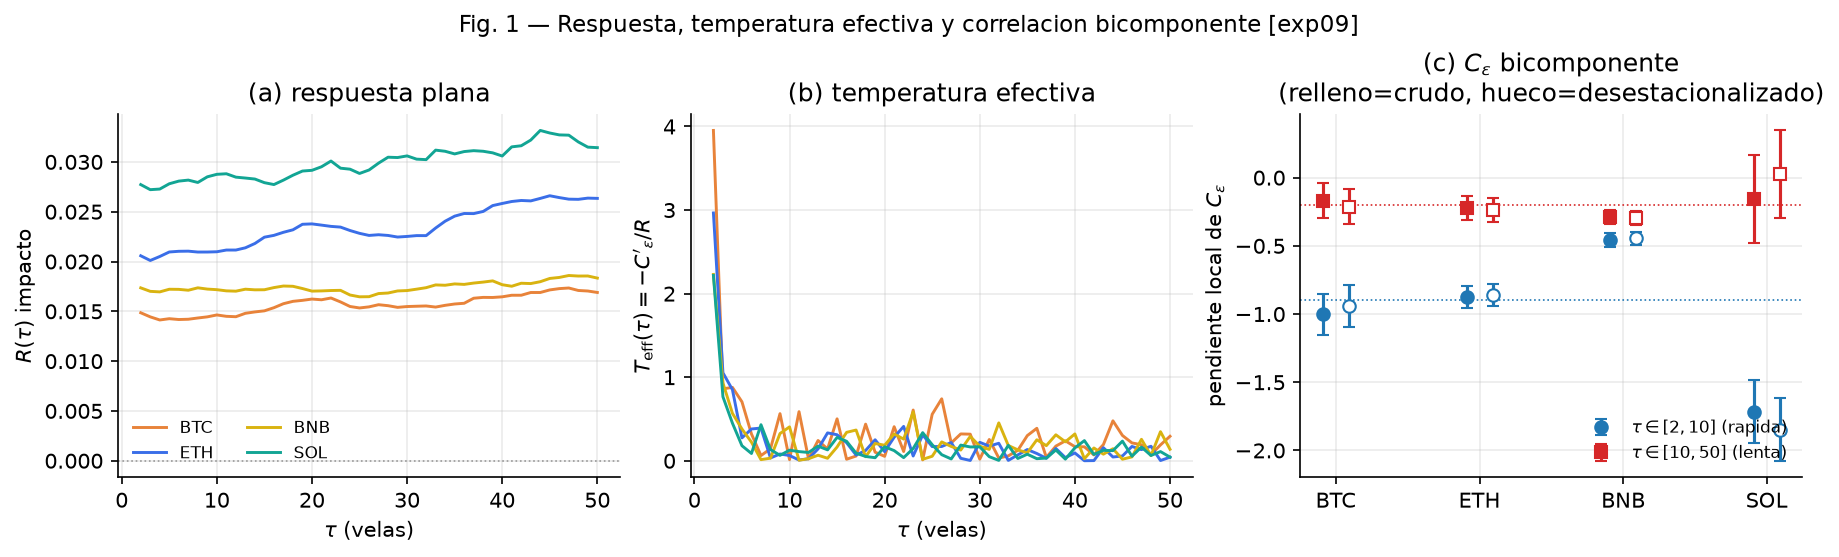
\includegraphics[width=\columnwidth]{../output/figuras/fig1_ceps_R_Teff.png}
  \caption{Base transport measurement at hourly resolution.
  (a) The impact response is nearly flat in lag.
  (b) The fluctuation--dissipation ratio $\Teff(\tau)$, which with flat $R$
  inherits its shape from $C'_\eps$.
  (c) Local decay exponents of $C_\eps$ in the fast and slow windows, raw
  (filled) and deseasonalised (open); removing the daily cycle does not move
  them, so the slow regime is not the drive.}
  \label{fig:base}
\end{figure}

\section{Counting statistics of the transferred flow}
\label{sec:counting}

We now count. Let $Q_T = \sum_{t=1}^{T}\eps_t$ be the flow transferred in a
window of $T$ candles, and let
\begin{equation}
  s(Q) \;=\; \ln\frac{P(Q_T = +Q)}{P(Q_T = -Q)}
\end{equation}
be its fluctuation symmetry function. In transport, linearity of $s$ with slope
$A$ is the signature of a driven steady state, and we follow the current
fluctuation theorem of Andrieux and Gaspard \cite{andrieux2007jsp} in calling
$A$ the \emph{affinity} --- the conjugate thermodynamic force of the counted
current, in the sense in which affinities arise from the cycle decomposition of
a Schnakenberg network.

\paragraph*{Two disclaimers on the name, both necessary.}
First, $A$ is not a temperature, and we avoid that word deliberately. At least
seven mutually incompatible ``market temperatures'' are already in print ---
from return log-ratios \cite{ramezani2025}, holding-time asymmetries
\cite{gao2026}, order-book energies \cite{li2024entropy}, Gibbs weights over
strategies, volatility-cascade bath couplings, index means, and the noise
parameter of minority games --- and none of them is a measured
fluctuation--response ratio. Adding an eighth would subtract clarity.

Second, and more seriously: $Q_T$ is a signed particle current, not an entropy
production, and the Gallavotti--Cohen symmetry is guaranteed only for the
latter. Barato and Chetrite \cite{barato2012} give the conditions under which a
\emph{non-entropic} current inherits a large-deviation function with the
Gallavotti--Cohen symmetry, and we do not establish that those conditions hold
here. We therefore treat the linearity of $s(Q)$ as a phenomenological
symmetry to be tested rather than a theorem to be confirmed, and the reader
should read $A$ as an operational slope with the dimensions of an affinity.
Sec.~\ref{sec:identity} makes the point sharper still: for a Gaussian $Q_T$
the linearity is not even phenomenological, but algebraic.

One consequence of this framing deserves flagging, because it constrains what
the two halves of this paper can independently claim. Andrieux and Gaspard
\cite{andrieux2007jstat} show that the fluctuation theorem for currents fixes
the response coefficients to arbitrary order from the fluctuations of the
accumulated currents, reducing near equilibrium to Green--Kubo. The affinity
of this section and the fluctuation--dissipation ratio of
Sec.~\ref{sec:response} are therefore not logically independent measurements,
and a relation between them is expected rather than surprising.

\subsection{An identity that must not be oversold}
\label{sec:identity}

Before reporting anything we state the caveat that governs how these results
should be read. For a Gaussian $Q_T$ with mean $m_T$ and variance $V_T$,
\begin{equation}
  s(Q) = \frac{(Q+m_T)^2-(Q-m_T)^2}{2V_T} = \frac{2m_T}{V_T}\,Q ,
  \label{eq:identity}
\end{equation}
exactly and always. A linear fluctuation symmetry whose slope equals
$2\avg{Q_T}/\Var(Q_T)$ is thus an \emph{algebraic identity}, not a physical
discovery, and observing it confirms only that the estimator and the moments
agree. We emphasise this because the surrounding literature makes it easy to
present such an observation as a fluctuation theorem, and it is not one.

Accordingly we report the closures below as consistency checks, and place the
weight of the paper on the quantities that Eq.~\eqref{eq:identity} cannot
account for.

\subsection{What closes}

The affinity exists and is far from the sign-randomised null in all eight
series. Splitting each series into four consecutive periods, the sign of $A$ is
stable across all four in BTC and ETH, and is at the noise level in BNB and
SOL; the taker flow is persistently net selling in BTC, ETH and SOL over the
sample. At $T=16$ hourly candles, $A = -1.550\pm0.098$ (BTC) and
$-0.576\pm0.074$ (ETH). The measured $A$ tracks $2\avg{Q_T}/\Var(Q_T)$ across
all windows [Fig.~\ref{fig:counting}(a)] --- which, by Sec.~\ref{sec:identity},
is exactly what it must do.

The second-order closure with the correlation sector is likewise clean: the
counting variance predicted from the independently measured $C_\eps$ agrees with
the observed one to within $4.6\%$ in the worst case, the ratio spanning
$0.954$ to $1.040$ over $64$ window--series combinations. The counting variance
adds no information beyond the autocorrelation. This is worth stating plainly
because it is often assumed otherwise.

Where the data have the statistical power to resolve it, the symmetry function
is linear: the cubic coefficient is $c_3 = 0.024\pm0.119$ for ETH$\cdot$1h at
$T=16$, consistent with zero. BTC$\cdot$1h shows $c_3 = 0.526\pm0.240$, a
$2.2\sigma$ curvature that we record without interpreting.

\subsection{What does not close}

Two things sit outside the Gaussian account.

First, the Fano factor is enormous. Because the carriers are trades drawn from
a broad size distribution, we normalise the counting variance to the Poisson
expectation for carriers of the typical size,
\begin{equation}
  \mathcal{F}(T)=\frac{\Var(Q_T)}{\bar q^{\,2}\,\avg{N_T}} ,
  \label{eq:fano}
\end{equation}
where $\bar q$ is the median traded volume per trade --- the effective transfer
quantum, taken as a median rather than a mean because the size distribution has
a heavy tail --- and $N_T$ is the number of trades in the window. A Poisson
stream of $N_T$ independent transfers of size $\pm\bar q$ gives
$\mathcal{F}=1$, so Eq.~\eqref{eq:fano} is the noise-to-Poisson ratio in the
usual transport sense and is what the free-fermion bound constrains. Referring
instead to the net transferred charge would divide by a nearly vanishing mean
and produce a number with no such interpretation.

Measured this way, $\mathcal{F}(T{=}1)$ ranges from $905$ to
$3342$ across the eight series [Fig.~\ref{fig:counting}(c)]. Its \emph{level}
is a statement about trade sizes --- a compound sum with a heavy-tailed size
distribution has $\mathcal{F}\sim\avg{q^2}/\bar q^{2}$, which is large for
reasons that have nothing to do with memory. Its \emph{growth} is a separate
statement: $\mathcal{F}$ increases as $T^{0.19}$ to $T^{0.28}$, and that
exponent does reflect memory and order splitting. Separating level from growth
is essential and, in our reading, not always done.

Second, the counting variance grows superdiffusively. Fitted over the whole
window grid the log-slope is $1.22\pm0.02$ to $1.37\pm0.02$ across series,
against $[0.90,1.14]$ for a permutation null that preserves the marginal
distribution but destroys memory.

The \emph{local} log-slope drifts upward with window size in every series, from
$1.14$--$1.27$ at the shortest windows to $1.45$--$1.56$ at the longest. We
report the drift but do not interpret it, because it is not identified. The
block variance is inflated by any drift in the per-block mean, which
contributes a term growing as $T^2$, and these series have such a drift: the
flow carries a persistent sell-side bias and modulates with the daily cycle
(Secs.~\ref{sec:counting} and~\ref{sec:floquet}). Estimators built from
vanishing-moment filters, which annihilate a constant, linear or quadratic
mean while preserving the exponent, return $\nu=1.10$--$1.36$ against
$1.31$--$1.43$ for the block estimator, lower in all four assets; injecting
each asset's own measured drift onto a synthetic series of known $\nu$ inflates
the block estimate by up to $0.13$ and leaves the filtered ones fixed; and
removing the drift by hand brings BTC from $1.42$ to $1.09$. What is robust is
the level, $\nu>1$ under every estimator --- superdiffusive growth, and hence
memory decaying more slowly than $\tau^{-1}$. The drift of the local exponent
is treated in the companion paper \cite{paper2}, where the same control is
applied to a prediction that rests on it. Two further caveats attach to the
long-window end. The number of non-overlapping windows falls as $T$ grows ---
at $T=256$ hourly candles only $137$ remain --- so those points are the
noisiest. And in BNB the local slope turns over rather than continuing to rise,
peaking near $1.48$ at $T=64$ and falling to $1.39$ by $T=256$ on the hourly
series. We do not know whether that turnover is a third regime or the
small-sample noise of the last few points, and we do not have the statistics to
decide.
No free-fermion counting problem produces this combination of a Fano factor of
order $10^3$ with sustained superdiffusive growth; the bunching must come from
interactions between flow and available liquidity.

\begin{figure}[t]
  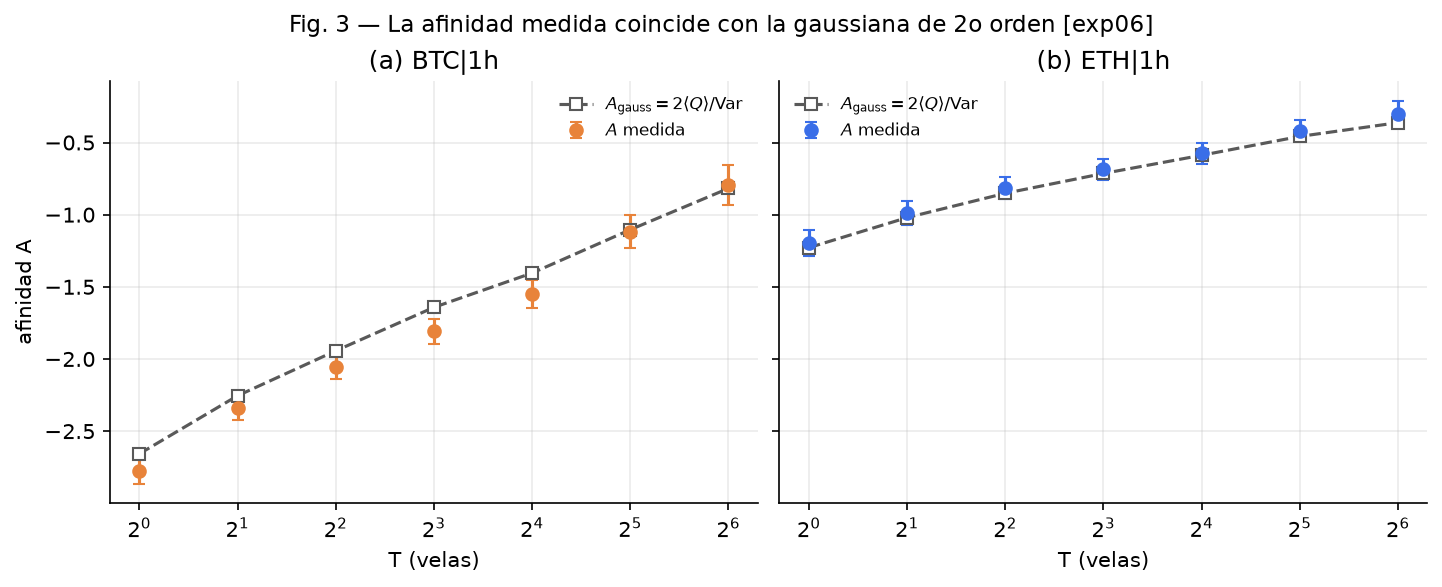
\includegraphics[width=\columnwidth]{../output/figuras/fig3_A_vs_Agauss.png}
  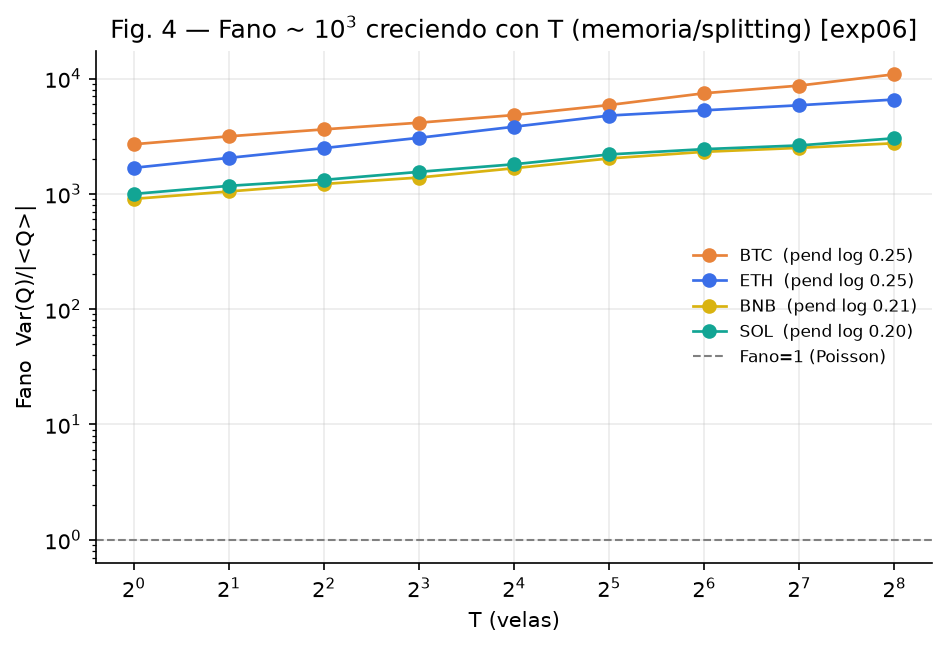
\includegraphics[width=\columnwidth]{../output/figuras/fig4_fano.png}
  \caption{Counting statistics. (a),(b) The measured affinity against the
  Gaussian value $2\avg{Q_T}/\Var(Q_T)$; agreement here is the identity of
  Eq.~\eqref{eq:identity}, not evidence of a fluctuation theorem.
  (c) The Fano factor, of order $10^3$ and growing with window size. The level
  reflects the heavy-tailed size distribution; the growth reflects memory.}
  \label{fig:counting}
\end{figure}

\section{Clocks: what ages after a shock, what does not, and what only appears
to}
\label{sec:clocks}

Systems with slow dynamics often age: correlation functions after a quench
depend on the time elapsed since the quench, not only on the lag. We tested this
directly, defining shocks as returns exceeding the $99.5$th percentile in
absolute value and building an ensemble of $240$ hourly post-shock trajectories.

The outcome of this section is easier to follow if we state it first. The mean
ages and the correlation does not --- but the correlation \emph{appears} to
age, strongly and monotonically, and the appearance survives every check except
the one that matters. The reason is a property of the estimator rather than of
the market: dividing a post-event signal by a quantity measured before the
event manufactures ageing by construction. We regard identifying that mechanism
and the null that exposes it as the more transferable of the two results, since
the construction it invalidates is in routine use.

The \emph{mean} normalised absolute return does relax with an age-dependent
profile of Omori form. We fit the \emph{amplitude} exponent $\beta$ in
$\sigma(t)\sim t^{-\beta}$ --- not the rate exponent $p$ in
$n(t) = K(t+\tau)^{-p}$, and the distinction matters because the two are
routinely conflated in this literature while being related by $p = \alpha\beta$
with $\alpha$ the tail index \cite{lillo2003}. Our conservative fit, excluding
the first few candles where the fast relaxation dominates, gives
$\beta = 0.61\pm1.01$; the error is large enough that the value carries little
weight on its own.

It is worth being explicit about where that sits. Published amplitude
exponents for equities cluster at $\beta \approx 0.22$--$0.32$
\cite{lillo2003,zawadowski2006}, so our point estimate is high by a factor of
two to three, although not resolved from them at this uncertainty. Read
instead as a rate exponent it would be unremarkable, falling in the mode of
the distribution over crashes reported by Selçuk \cite{selcuk2004}. The
internal consistency check available here is $p = \alpha\beta$: with a tail
index of order $3$, an amplitude exponent near $0.2$ would follow from a rate
exponent near $0.6$. We report the amplitude fit because that is the quantity
we measured, and we do not convert.

The correlation time $\tau_c(t_w)$ also appears to grow with age,
monotonically, with a Spearman coefficient of $+1.00$ across age bins.

That second result is an artefact, and the way we caught it generalises. Placing
shocks at \emph{random} times and repeating the whole analysis, the null
ensemble returns a median Spearman coefficient of $+1.00$ as well
[Fig.~\ref{fig:clocks}]. The cause is the pre-event normalisation: dividing by
the volatility measured just before the event injects a slow common mode,
because the volatility drifts away from its pre-event value as age increases,
and this manufactures apparent ageing for \emph{any} clock, including a
meaningless one. The observed growth is statistically indistinguishable from
that artefact, so we report no ageing in the correlation.

We state the resulting rule in general form, because the construction that
produces it is not unusual: \emph{in any event-conditioned two-time analysis,
normalising by a pre-event quantity fabricates ageing, and a null built from
randomly placed events is mandatory rather than optional.} The null costs one
re-run of the same pipeline, which is a small price for a result that would
otherwise be a discovery.

\paragraph*{Why we think this generalises.}
The mechanism is not specific to markets, and versions of each half of it are
established elsewhere. That normalising by a noisy denominator biases an
estimator is old \cite{pearson1897,kronmal1993}; the sharpest modern statement
is that the bias is controlled by the correlation between numerator and
denominator \cite{ciuparu2016}, which in our geometry decays with $t_w$ and so
generates a profile in age rather than a constant offset. That conditioning on
an extreme value inflates a subsequently measured correlation is the
Forbes--Rigobon effect \cite{forbes2002,boyer1999}, where an event-selected
variance in the denominator changes a measured cross-market correlation from
$0.45$ to $0.81$ with no change in the data-generating process; what we
describe is its two-time analogue. And the scaling argument itself has been
made exactly, in another system: for a granular fluid in the homogeneous
cooling state, Brey \textit{et al.}\ \cite{brey2007} show that normalised
two-time correlation functions decay more slowly the later the measurement
begins, purely because the overall scale of the signal decays self-similarly,
with no memory whatever --- and that the effect disappears in properly
rescaled variables.

Two alternative explanations must be excluded rather than assumed away. The
sample autocorrelation is biased in finite samples \cite{kendall1954}, and the
resulting bias in a fitted decay time grows with record length --- but that
bias is negative, depends on the number of points rather than on the age, and
is present in our randomly placed null as well, so it cannot produce a
difference between the two \cite{zeraati2022}. Separately, a time-averaged
correlation function computed from a trajectory shorter than the longest
relaxation time shows apparent ageing on its own \cite{akimoto2023}; our
placebo controls for this for the same reason.

\paragraph*{Scope of the claim.}
We want to be careful about how far this reaches. What we have shown is that
\emph{in our data}, with our normalisation, the measured growth of $\tau_c$
with age is indistinguishable from what randomly placed events produce. That
is a statement about this measurement, and it does not by itself invalidate
any other.

It does, however, apply to a construction used elsewhere. The same object --- a
$\sigma$-normalised two-time correlator built on event-conditioned windows,
with the waiting time counted from the conditioning event --- underlies reports
of ageing in aftershock sequences and, subsequently, in a currency crash
\cite{abe2004,usmanova2017}. We are not aware of a published null of this kind
for those analyses. Whether the effect reported there survives such a null is a
question we cannot settle with market data and do not attempt to settle here;
we raise it because the check is cheap and, on our data, decisive. The
normalisation convention $C(t,t_w)/C(t_w,t_w)$ is standard in the ageing
literature, and Brey \textit{et al.}\ \cite{brey2007} show analytically that
this convention alone produces full ageing in a system with no memory, which
suggests the question is worth asking generally rather than only here.

\begin{figure}[t]
  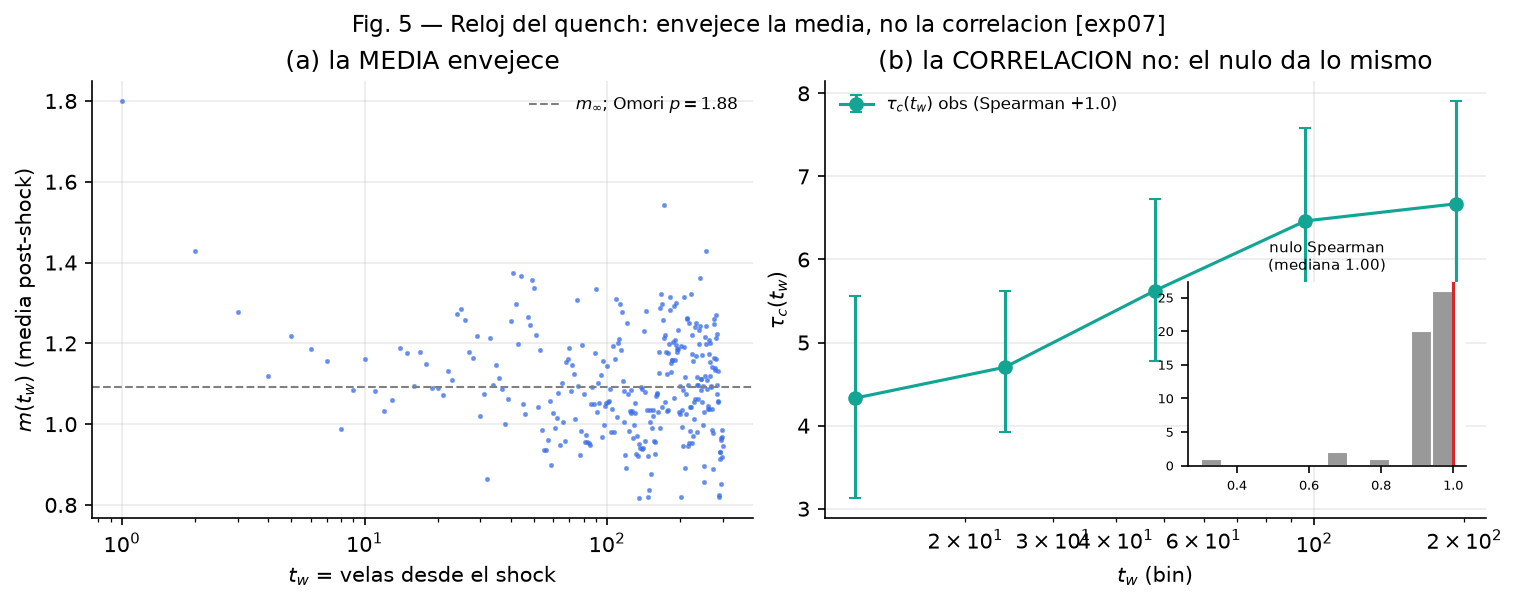
\includegraphics[width=\columnwidth]{../output/figuras/fig5_reloj_quench.png}
  \caption{Post-shock behaviour. (a) The mean flow relaxes with age.
  (b) The correlation time appears to grow with age, but randomly placed
  shocks reproduce the same monotone growth (inset), identifying it as an
  artefact of pre-event normalisation.}
  \label{fig:clocks}
\end{figure}

\section{The driven conductor}
\label{sec:floquet}

Markets run on a daily cycle, so the natural question is whether the transport
coefficients themselves --- not merely the activity --- modulate with the phase
of that cycle. Binning by hour of day and comparing against a null that rotates
the phase labels day by day (which preserves within-day structure while
destroying its alignment to clock time), we find that the bias, the affinity and
the impact all modulate significantly in all four assets at hourly resolution,
each at the smallest empirical $p$ the $K=50$ null can resolve, $p=0.020$. The
four-hourly series reproduce this. The Fano factor modulates in only two of four
assets and we treat it as unresolved.

As a positive control we included the raw activity, which is known to have
strong daily seasonality and which the procedure must therefore detect; it does,
in all four assets. This matters: a null result on a phase analysis is
uninterpretable without evidence that the machinery can see a modulation that
is certainly there.

The profile itself is coherent across assets [Fig.~\ref{fig:floquet}]: the
selling imbalance and the affinity both peak during the Asian night, while the
impact nearly doubles during the European--US overlap. The market is not a
steady-state conductor with a constant bias; it is a periodically driven one,
and any model that omits the drive is incomplete.

\begin{figure}[t]
  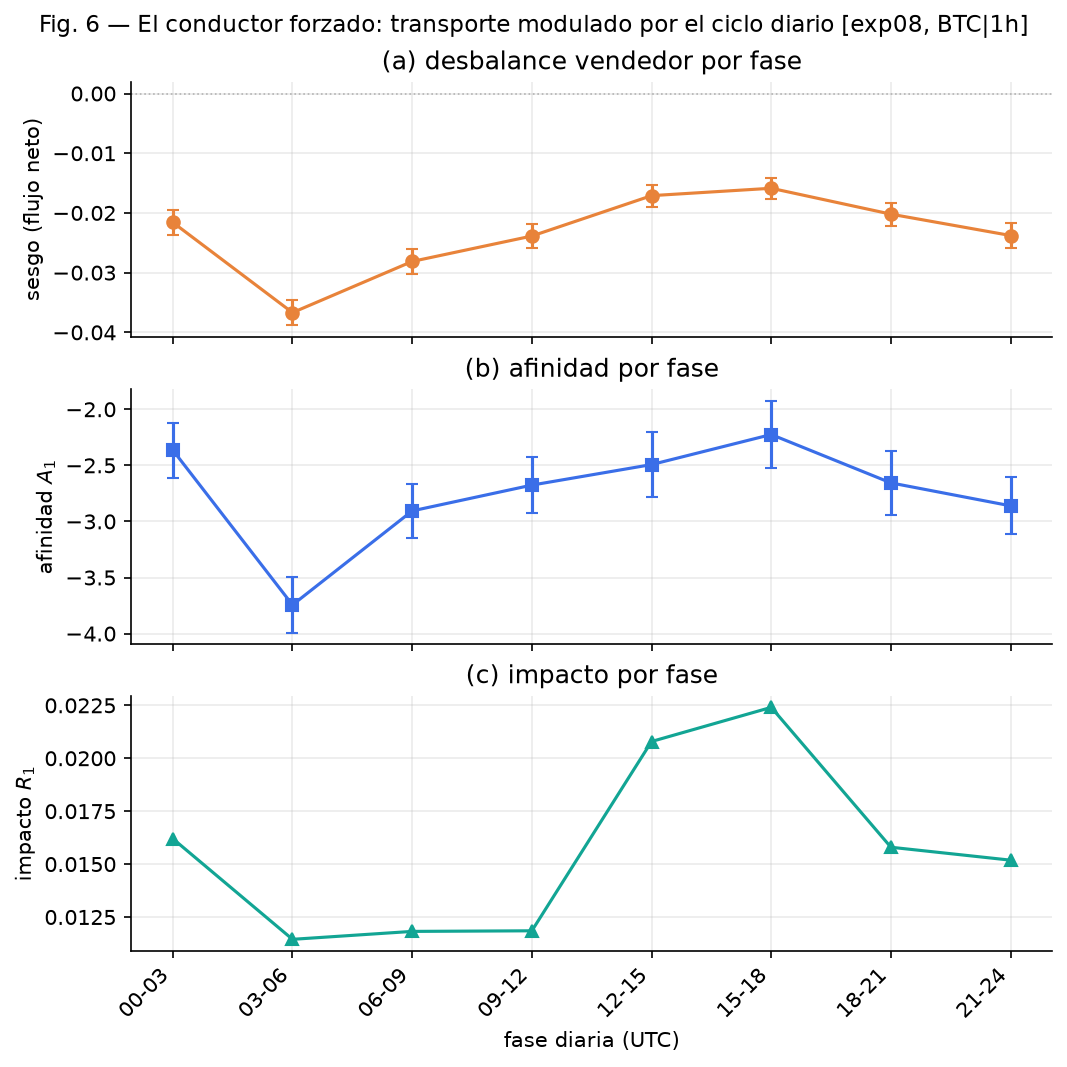
\includegraphics[width=\columnwidth]{../output/figuras/fig6_floquet_perfiles.png}
  \caption{Transport coefficients as functions of daily phase (BTC, hourly):
  (a) net flow bias, (b) affinity, (c) impact. All three modulate
  significantly against a phase-rotation null.}
  \label{fig:floquet}
\end{figure}

\section{Methods and statistical caveats}
\label{sec:methods}

Three inference problems arose that we think are worth reporting on their own,
because each of them produced, at some stage, a result we would otherwise have
believed.

\paragraph*{Predictive comparison is miscalibrated under heavy tails, unevenly.}
Comparing forecast accuracy with the standard Diebold--Mariano test
\cite{diebold1995} using Newey--West standard errors \cite{neweywest1987}, we
generated the null distribution by permutation through the identical pipeline.
The empirical rejection rate at nominal $5\%$ is $4$--$6\%$ for BTC but
$16$--$18\%$ for ETH, with a null standard deviation of about $2.1$ instead of
$1.0$. A nominal $p<0.05$ on the heavier-tailed asset is worth roughly $0.17$.
The practical consequence is that nominal $p$ values must not be compared across
assets as though they measured the same thing.

\paragraph*{Scanning scales without maxT manufactures findings.}
Sweeping $144$ configurations (assets $\times$ intervals $\times$ windows
$\times$ horizons $\times$ baselines) and applying the Westfall--Young maxT
correction \cite{westfall1993}, the best cell had a nominal $p$ of
$2\times10^{-4}$ --- and yet the maximum statistic generated by chance over
those same $144$ cells had a mean of $3.775$, \emph{above} the observed maximum
of $3.667$. The global $p$ was $0.43$. Only five cells passed $p<0.05$ where
$7.2$ would be expected by chance. Without the correction this would have been
published as a discovery. Bonferroni is not an adequate substitute, since the
cells share data and are far from independent.

\paragraph*{Recalibration is not information, and correlation is not evidence.}
A model $\log(\mathrm{rv}) \sim a + b\log\sigma + cX$ beats raw $\sigma$ even
when $X$ is pure noise, because it re-fits level and slope; the contrast that
decides must always be recalibrated-without-$X$ against recalibrated-with-$X$.
Relatedly, a pure AR(1) noise feature with no relation to the data correlated
with out-of-sample $\log(\mathrm{rv})$ at $+0.21$ (BTC) and $+0.32$ (ETH) ---
higher than the real feature. Spurious correlation between persistent series is
the rule, not the exception.

\paragraph*{Negative results need positive controls.}
Surrogate and permutation nulls demonstrate that a pipeline does not manufacture
signal. None of them demonstrates that it can \emph{see} a signal. Every
negative result reported here is accompanied by a positive control on synthetic
data carrying the effect by construction, without which a null is ambiguous
between ``no effect'' and ``broken code''. This is the standard requirement of
assay sensitivity \cite{ich2000}, transposed to a computational pipeline as an
injection--recovery test; we note it because retrospective power computed from
an observed effect size is not a valid substitute \cite{hoenig2001}.

\paragraph*{The memory exponent is estimator-dependent, and the disagreement is
itself the measurement.}
Lillo and Farmer \cite{lillo2004} obtain $\gamma=0.39$ by log--log regression on
the sample autocorrelation and $0.61$ by periodogram \emph{on the same data},
and state that the sample autocorrelation is a poor estimator of $\gamma$. We
therefore computed $\gamma$ four ways --- log--log regression on $C_\eps$, a
log-periodogram (GPH) regression, detrended fluctuation analysis, and the
wavelet log-scale diagram of Abry and Veitch
\cite{abry1998,veitch1999}. The last plots $\log_2\langle d_j^2\rangle$ against
octave $j$, where $d_j$ are Daubechies detail coefficients; for a process with
$C_\eps(\tau)\sim\tau^{-\gamma}$ the diagram is a straight line of slope
$\alpha=1-\gamma$. Two properties make it the natural arbiter here. A Daubechies
filter with $L/2$ vanishing moments annihilates polynomial trends of degree
below $L/2$ \cite{daubechies1992}, so a drifting mean cannot masquerade as
memory; and the details are close to decorrelated across octaves for
self-similar input \cite{flandrin1992}, so the fit returns an error bar and a
goodness-of-fit for the power law it assumes --- which the other three do not.

All four were calibrated against series with $\gamma$ known by construction. The
choice of calibration series is not a detail: an estimator that reads the
low-frequency end of the spectrum cannot be validated against a generator whose
autocovariance is matched only at short lags, since the approximation error then
sits precisely in the band being measured. We therefore synthesise exact
fractional Gaussian noise by the circulant method of Davies and Harte
\cite{davies1987}, whose spectral factorisation is exact for the fGn
autocovariance and needs no eigenvalue truncation. Over $\gamma\in[0.4,0.8]$
with $4\times10^5$ samples, the mean absolute errors are $0.011$ (wavelet),
$0.023$ (DFA), $0.026$ (regression) and $0.068$ (GPH). No estimator is grossly
biased and the wavelet is the most accurate, so the disagreement seen on real
data cannot be attributed to any one of them being broken.

On our data the four spread by $0.23$ (BNB) to $0.53$ (SOL), an order of
magnitude beyond what the calibration allows for estimator noise. The wavelet
diagnostic supplies the reason: the log-scale diagram is not straight. A
single-slope weighted fit over $j\ge3$ returns $\chi^2$ per degree of freedom of
$3.7$, $1.9$, $3.1$ and $6.1$ for BTC, ETH, BNB and SOL, rejecting the
single-power-law model outright. There is therefore no single $\gamma$ for the
four estimators to agree on: each returns a different weighted average over
scales, according to where in the spectrum it places its weight. This is the
same conclusion the two-window fit of Sec.~\ref{sec:acf} reaches from the
autocorrelation, arrived at independently and with an explicit goodness-of-fit
rather than by comparing two fitted ranges. The values in Sec.~\ref{sec:acf}
should accordingly be read as a band of roughly $\pm0.1$ rather than as
three-decimal measurements, and the same caution applies to any published
exponent quoted from a single estimator without the goodness-of-fit of the power
law it presumes. The resolvable range is set by the record: $3.5\times10^4$
hourly observations give about nine usable octaves, and beyond $j=8$ fewer than
$130$ coefficients survive, so the slow component sits at the edge of what these
series can resolve at all.

The exponent is also not stable across data vintages: restricting the same
series to its most recent two years gives $\gamma=0.610\pm0.097$ for BTC
against $0.380\pm0.052$ over four years. We report the four-year values
throughout and flag the instability rather than selecting the vintage that
agrees best with the literature.

\paragraph*{The phase modulation is not an aggregation artefact.}
Barardehi and Bernhardt \cite{barardehi2025} show that calendar-time
aggregation, when trading intensity itself varies with the time of day,
produces an over-aggregation bias sufficient to manufacture intraday patterns
in volatility and in Kyle's lambda. Since activity in our data modulates by a
factor of about $1.9$ across the daily cycle, the impact modulation of
Sec.~\ref{sec:floquet} is exposed to exactly this objection. We repeated the
measurement on two other clocks. Restricting every phase bin to candles whose
trade count falls inside a band common to all phases --- so that activity is
matched by construction --- the max/min ratio of $R(1)$ across phase is $1.53$
to $1.86$ across the four assets, against $1.56$ to $1.98$ in calendar time.
Aggregating consecutive candles into bars of approximately constant trade count
gives $1.35$ to $1.67$. The modulation attenuates but survives on both clocks,
so it is not produced by aggregation. We note the limitation that public candle
data carry only a trade count, so the second clock is a coarse trade clock
rather than a true one.

\paragraph*{Finite-sample autocorrelation bias cannot explain the apparent
ageing.} A second mechanism could in principle produce the artefact of
Sec.~\ref{sec:clocks}: the sample autocorrelation is biased in finite samples
\cite{kendall1954}, and a fitted correlation time therefore grows with the
number of points available. We quantified it on AR(1) processes with known
$\rho$: at $\rho=0.95$ the fitted $\tau$ recovers $32\%$ of its true value at
$n=50$ and $97\%$ at $n=1600$, so the effect is large enough to matter. It
cannot act here, however, because the ensemble size entering each correlation
estimate is the number of shocks and is therefore constant in the age $t_w$ ---
we verified this directly, with a relative range across age bins of exactly
zero for all four assets. A bias that does not vary with $t_w$ cannot generate
a profile in $t_w$. It is also present in the randomly placed null, which
controls for it in any case.

\section{Discussion}
\label{sec:discussion}

Read as a conductor, the market separates into three sectors with three
different statuses, and we think this separation is the most useful output of
the measurement.

The \emph{second-order sector} is closed and, in a precise sense, empty: the
counting variance is the autocorrelation, the affinity is
$2\avg{Q}/\Var(Q)$, and the phase dependence of the affinity follows from the
first two moments. All of this is consistency, not physics, for the reason given
in Sec.~\ref{sec:identity}.

The \emph{response sector} is explained: with the price integrating the
unpredictable part of the flow, the impact is flat and the
fluctuation--dissipation ratio inherits its shape from $C'_\eps$. The measured
``violation'' is a shape, not a mystery.

The \emph{counting sector} is open, and it is where the physics is. A Fano
factor of order $10^3$ with sustained superdiffusive growth of the variance is
outside what free-fermion counting can produce, which locates the missing
ingredient in interactions between order flow and latent liquidity rather than
in the Gaussian transport sector. The two-regime correlation function points the
same way, with the slow component matching the multi-day scale of order
splitting \cite{lillo2005,sato2023prl}.

Two further findings constrain any model. The mean ages after a shock while the
correlation does not, so a model needs bath memory but not genuine ageing of its
kernel. And the transport coefficients modulate with the daily cycle in every
asset we tested, so periodic driving is a required ingredient, not a refinement.

\paragraph*{What the bunching implies.}
Of the three sectors, only one carries information that is not already in the
correlation function, and it points somewhere specific. A Fano factor of
$10^{3}$ is a statement about the distribution of transfer sizes: a compound
process with heavy-tailed sizes gives $\mathcal{F}\sim\avg{q^{2}}/\bar q^{2}$,
which is large for reasons unconnected to memory. Superdiffusive growth of the
variance is a statement about memory, and follows from a correlation decaying
more slowly than $\tau^{-1}$. The two requirements are separable, and together
they say that a model of this market needs a marked point process with heavy
tails \emph{and} a two-component kernel --- not one or the other. That both
requirements survive the transport reading, while everything else in the
second-order sector collapses into identities, is the reason we think the
counting layer is worth adding to the standard microstructure toolkit.

\paragraph*{A negative result we consider part of the finding.}
We began this work asking whether two-time structure imported from
nonequilibrium field theory would improve volatility forecasting, and it does
not. Across five pre-registered designs --- correlation-based features,
response--correlation ratios, a $144$-cell scale sweep, a change of target from
conditional mean to tail probability, and stretched-exponential relaxation
parameters fitted window by window --- nothing survived correction for multiple
comparisons, with global $p$ values of $0.43$ and $0.20$ for the two best-powered
designs. In one instance the same asset produced significant effects in opposite
directions at two resolutions, which we regard as more decisive than any $p$
value. The diagnostics are real, and they are informative about the market's
transport structure; they are simply not predictive of the second moment at
these scales. We report this because the measurement programme above is what
survived, and readers deserve to know what did not.

\begin{acknowledgments}
\end{acknowledgments}

\bibliography{refs}

\end{document}
